% Created 2024-04-19 Fri 09:59
% Intended LaTeX compiler: pdflatex
\documentclass[letterpaper, 10pt, twocolumn]{article}
                      \usepackage{lmodern} % Ensures we have the right font
\usepackage[T1]{fontenc}
\usepackage[utf8]{inputenc}
\usepackage{graphicx}
\usepackage{amsmath, amsthm, amssymb}
\usepackage[table, xcdraw]{xcolor}
\renewcommand{\thesection}{\Roman{section}}
\renewcommand{\thesubsection}{}
\renewcommand{\thesubsubsection}{}
\definecolor{bblue}{HTML}{0645AD}
\usepackage[colorlinks]{hyperref}
\hypersetup{colorlinks, linkcolor=blue, urlcolor=bblue}
\usepackage{titling}
\setlength{\droptitle}{-6em}
\setlength{\parindent}{12pt}
\setlength{\parskip}{0em}
\usepackage[stretch=10]{microtype}
\usepackage{hyphenat}
\usepackage{ragged2e}
\usepackage{subfig} % Subfigures (not needed in Org I think)
\usepackage{hyperref} % Links
\usepackage{listings} % Code highlighting
\usepackage[top=1in, bottom=1.00in, left=1in, right=1in]{geometry}
\renewcommand{\baselinestretch}{1.00}
\usepackage[explicit]{titlesec}
\pretitle{\begin{center}\fontsize{20pt}{20pt}\selectfont}
\posttitle{\par\end{center}}
\preauthor{\begin{center}\vspace{-6bp}\fontsize{14pt}{14pt}\selectfont}
\postauthor{\par\end{center}\vspace{-25bp}}
\predate{\begin{center}\fontsize{12pt}{12pt}\selectfont\vspace{1em}}
\postdate{\par\end{center}\vspace{0em}}
\titlespacing\section{0pt}{5pt}{5pt} % left margin, space before section header, space after section header
\titlespacing\subsection{0pt}{5pt}{-2pt} % left margin, space before subsection header, space after subsection header
\titlespacing\subsubsection{0pt}{5pt}{-2pt} % left margin, space before subsection header, space after subsection header
\usepackage{enumitem}
\setlist{itemsep=-2pt} % or \setlist{noitemsep} to leave space around whole list
\usepackage{listings}
\onecolumn
\twocolumn
\author{Jackson Mowry}
\date{4/16/24}
\title{\textbf{Maximizing Requests per Second on a Single Thread through \texttt{io\_uring}}}
\hypersetup{
 pdfauthor={Jackson Mowry},
 pdftitle={\textbf{Maximizing Requests per Second on a Single Thread through \texttt{io\_uring}}},
 pdfkeywords={},
 pdfsubject={},
 pdfcreator={Emacs 28.0.92 (Org mode 9.6)}, 
 pdflang={English}}
\begin{document}

\maketitle

\section{Abstract}
\label{sec:org5d8015c}
\textbf{This research paper investigates the transformative potential of io\textsubscript{uring} in scaling HTTP web servers to accommodate the needs of numerous concurrent clients. Despite the extensive exploration of various scaling techniques, little attention has been paid to the potential paradigm shift that \texttt{io\_uring} may introduce in asynchronous I/O architectures. \texttt{io\_uring} enables the handling of workloads traditionally confined to highly parallelized systems. This paper aims to explore the implications of \texttt{io\_uring} on asynchronous I/O systems, shedding light on its promise for enhancing server scalability and performance in the face of ever increasing demands.}

\section{Introduction}
\label{sec:org8f7dc37}
Web servers are a piece of software that sit between nearly every interaction a client makes on their device, and access to the files housed on a server. Despite this fact they are rarely inovated on, due to the fact that for most use cases they are ``good enough''. It is true that even a naive HTTP server can serve thousands of requests per second, which easily surpasses the needs of most users. The same architecture can be transplanted on top of a machine with many CPU cores in order to scale up to meet demands.

But these workloads are still inhrently synchronous at some level (excluding \texttt{aio}). \texttt{io\_uring} brings a true asynchronous io system to the table with its introduction into the Linux kernel (version 5.1).

In this article we will explore ``\href{https://wiki.c2.com/?IoMultiplexing}{multiplexed io}'' on linux through the use of \texttt{io\_uring}. Implementations are compared to the best possible implementation on a single core under other programming models. Along with single core tests we will pit our single core against a threaded server.

\section{Asynchronous IO}
\label{sec:org1be8050}
Most if not all system calls used in day to day software are considered ``blocking'', meaning they will only return once the entire function has finished executing. This model allows for programs to not having to worry about order of execution, as they know their program will run top to bottom without skipping a step. However, large web servers simply cannot afford to spend the time waiting for each system call to execute to completion. To avoid this problem of blocking programmers may choose to design their software around asynchronous IO.

On Linux this has taken the form of \texttt{epoll}, which allows for certain operations to be performed without blocking the main thread of execution.

\section{\texttt{aio}}
\label{sec:org4bc1363}
The \texttt{aio} system in Linux has two implementations, POSIX compliant, and the Linux implementation. Both systems suffer the same issue, they are intended to work with regular files, and as such don't play well with sockets. glibc creates a thread pool to perform regular synchronous io off the main thread, giving the illusion of asynchronosity.

For all of these reasons \texttt{aio} is generally avoided in application code.

\section{\texttt{epoll}}
\label{sec:orgeed39ab}
\texttt{epoll} is kernel based implementation of \texttt{poll}, with both providing a way to monitor a range of file descriptors, and alerting the user when one or many are ready for IO. It has become a very common architecture for web servers and other asychronous io systems to be built on top of. Most notably to implement the primatives golang's \texttt{net/http} package is built upon, and \texttt{libuv} which powers the Node.js event loop.

\texttt{epoll} expands on the original ideas of poll by sharing a list of file descriptors between the user and kernel, preventing the need for data to be copied back and forth. When any number of file descriptors are ready for IO they will be placed in a separate shared list, which the user can then perform the desired action on.

This architecture allows for a single thread to handle large numbers of active file descriptors, only slowing down to perform the synchronous operations like reading or writing. The actual implementation does not allow for asynchronous sending or recieving of data, merely alerting the user when those operations can be performed without blocking.

One downside of \texttt{epoll} is that it does not behave consistently across file descriptors of different types. While it is true that recieving data from a socket can block, which \texttt{epoll} is aware of, regular files do not exhibit the same behavior. On Linux read and write calls to a file should not block, but as we all know this is not true. You can make a write call and expect it to complete instantly, but if the kernels write cache is full, you will have to wait. The same goes for a read call which can blocked if the file is on a slow drive.

\section{\texttt{io\_uring}}
\label{sec:org5ddc2c8}
\texttt{io\_uring} is the latest attempt at adding asynchronous operations to Linux. Its design makes it obvious that it the designer learned from many of the shortcomings of \texttt{aio}. Not only does \texttt{io\_uring} provide a common interface across all types of file descriptors, it also implements most systems calls in an asyncronous fashion.

The design can be broken down into two distinct parts, a job submission queue, and a job completion queue, both implemented via ring buffers shared between the kernel and user space. At a basic level each submission is a combination of an op code defining which system call to perform, and the associated arguments. If the user desires to keep track of a job they can associate user data with a submission, which takes the form of an 64-bit integer, commonly used to hold a pointer. The implementation garuntees that user data will not be modified.

Once a job is complete it is placed in the completion queue, which an application can pull from. Completions have 2 main fields to pay attention to: a result code, and the associated user data. The result code is analogous to the return value from regular blocking system calls with one exception. Due to the concurrent execution of submissions the system cannot garuntee that the \texttt{ERRNO} associated with each system call will still be properly set when a user recieves a completion. Instead, \texttt{ERRNO} is placed in the completion struct, with its value negated so that it will not be confused with a successful execution.

\texttt{io\_uring} also offers one distinct advantage over the other asynchronous io methods presented here. Jobs can be submitted through a system call, or by having the kernel continuously poll the submission queue using a separate thread. This allows for a program to operate entirely in user space, avoiding system calls which have become even more costly in the age of speculative execution mitigations. We will explore both methods of job submission to see where their advantages lie.
\section{Methods}
\label{sec:org2e56d5e}
Testing will include an \texttt{epoll} server, two distinct \texttt{io\_uring} servers, and a fourth synchronous server using \texttt{poll}. Servers will parse a request, open a file, respond with the appropriate headers, send the file, and finally close the connection. Performance testing using \texttt{wrk} at \{1, 4, 8, 16, 32, 64, 128, 256, 512, 1024, 2048, 4096, 8192\} concurrent connections run over 30 seconds, with the mean of 3 runs reported for each metric.
\section{Results}
\label{sec:orgfdf92ae}
\begin{center}
\includegraphics[width=.9\linewidth]{p99_latency.png}
\end{center}
\begin{center}
\includegraphics[width=.9\linewidth]{mbps.pn.png}
\end{center}
\begin{center}
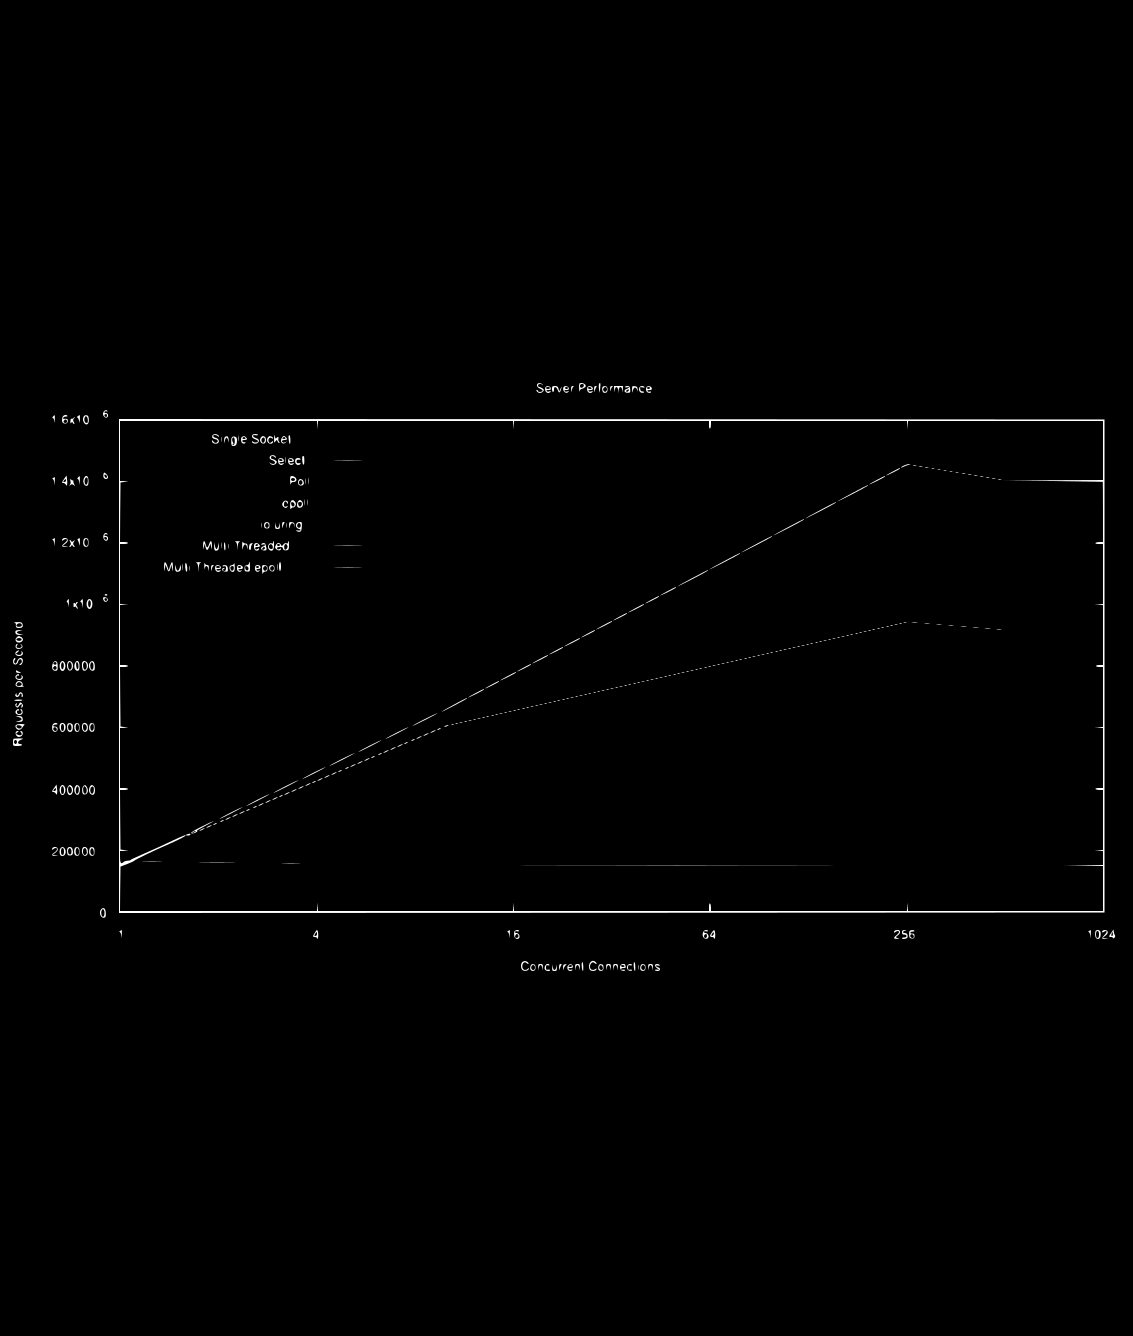
\includegraphics[width=.9\linewidth]{rps.png}
\end{center}
\section{Discussion}
\label{sec:org746c72e}
\section{Cite}
\label{sec:orgf73fe28}
\url{https://www.kernel.org/doc/ols/2003/ols2003-pages-351-366.pdf}
\url{https://www.landley.net/kdocs/mirror/ols2004v1.pdf\#page=215}
\url{https://darkcoding.net/software/linux-what-can-you-epoll/}
\url{https://darkcoding.net/software/epoll-the-api-that-powers-the-modern-internet/}
\end{document}
